%Docmment Class
\documentclass[12pt,report]{article}

%Packages
\usepackage{titlesec}
\usepackage{blindtext}
\usepackage{microtype}
\usepackage{booktabs}
\usepackage{placeins}
\usepackage{enumitem}
\usepackage{xcolor}
\usepackage{xhfill}
\usepackage{multicol}
\usepackage{float}
\usepackage{url}
\usepackage[hidelinks]{hyperref}
\usepackage[margin=0.5in]{geometry}
\usepackage{graphicx}
\usepackage{tikz}

%Formating for Control Logic Process Diagram
\tikzstyle{startstop} = [rectangle, rounded corners, text width = 15cm, minimum height=1cm, text centered, draw=black, fill=red!30]
\tikzstyle{io} = [trapezium, trapezium left angle=70, trapezium right angle=110, minimum width=3cm, minimum height=1cm, text centered, draw=black, fill=blue!30]
\tikzstyle{process} = [rectangle,text width = 19cm, minimum height=1cm, text centered, draw=black, fill=orange!30]
\tikzstyle{arrow} = [thick,->,>-stealth]


%Section Formatting
%\titlespacing{\section}{0pt}{*1}{*1}

\titleformat{\section}
    {\LARGE\bfseries}{\filright\footnotesize\enspace SECTION\thesection\enspace}{12pt}
    {\titlerule[1.6pt]}

\titleformat{\subsection}
    {\large\bfseries}{\thesection}{1em}{}
    % [{\titlerule[0.8pt]}]

\setlength{\parindent}{0pt}%

\pagenumbering{gobble}
\date{}

\begin{document}

\section*{Github - Procedures}

The purpose of this document is provide guidance for basic github usage: pushing code onto a remote repo efficiently on Linux based system predominantly from the command line.

\subsection*{Creating Local Repository and Connecting to Remote Repository}

\begin{figure}[H]
	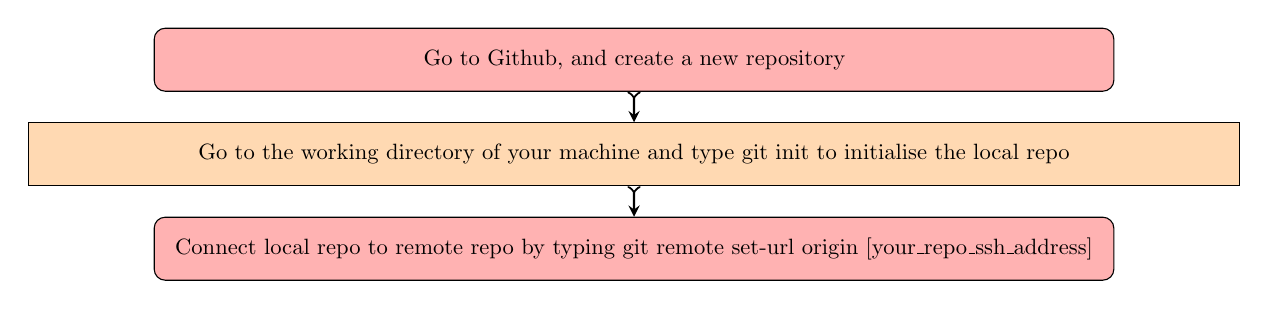
\begin{tikzpicture}[node distance = 1.5cm,every node/.style={scale=0.8}]

	\node (start) [startstop] {Go to Github, and create a new repository};
	\node (init) [process,below of=start] {Go to the working directory of your machine and type git init to initialise the local repo};
	\node (remote) [startstop,below of=init] {Connect local repo to remote repo by typing git remote set-url origin [your\_repo\_ssh\_address]};

	\draw [arrow] (start) -- (init){};
	\draw [arrow] (init) -- (remote) {};

\end{tikzpicture}
\centering
\end{figure}

\subsection*{Creating SSH Keys for Authentication Protocol}

\begin{figure}[H]
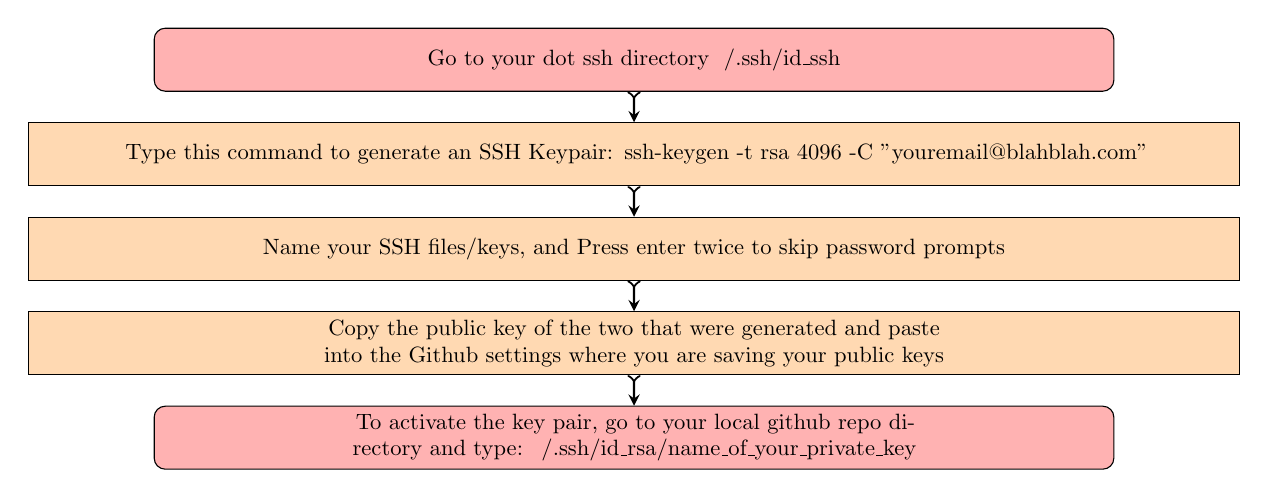
\begin{tikzpicture}[node distance = 1.5cm,every node/.style={scale=0.8}]

	\node (start) [startstop] {Go to your dot ssh directory \url{~}/.ssh/id\_ssh};
	\node (keygen) [process,below of=start] {Type this command to generate an SSH Keypair: ssh-keygen -t rsa 4096 -C "youremail@blahblah.com"};
	\node (skip) [process,below of=keygen] {Name your SSH files/keys, and Press enter twice to skip password prompts};
	\node (pub) [process,below of=skip] {Copy the public key of the two that were generated and paste into the Github settings where you are saving your public keys};
	\node (activate) [startstop,below of=pub] {To activate the key pair, go to your local github repo directory and type: \url{~}/.ssh/id\_rsa/name\_of\_your\_private\_key};

	\draw [arrow] (start) -- (keygen){};
	\draw [arrow] (keygen) -- (skip) {};
	\draw [arrow] (skip) -- (pub) {};
	\draw [arrow] (pub) -- (activate) {};

\end{tikzpicture}
\centering
\end{figure}

\subsection*{Pulling Repo Latest Revision then Commiting and Pushing Changes}


\begin{figure}[H]
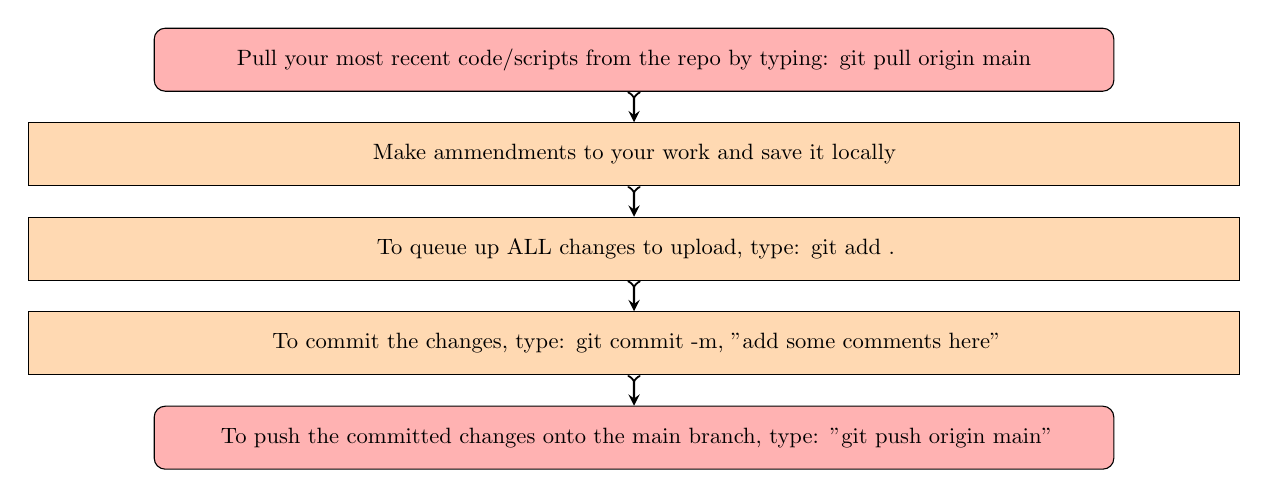
\begin{tikzpicture}[node distance = 1.5cm,every node/.style={scale=0.8}]

	\node (start) [startstop] {Pull your most recent code/scripts from the repo by typing: git pull origin main};
	\node (work) [process,below of=start] {Make ammendments to your work and save it locally};
	\node (add) [process,below of=work] {To queue up ALL changes to upload, type: git add .};
	\node (commit) [process,below of=add] {To commit the changes, type: git commit -m, "add some comments here"};
	\node (push) [startstop,below of=commit] {To push the committed changes onto the main branch, type: "git push origin main"};

	\draw [arrow] (start) -- (work){};
	\draw [arrow] (work) -- (add){};
	\draw [arrow] (add) -- (commit){};
	\draw [arrow] (commit) -- (push){};


\end{tikzpicture}
\centering
\end{figure}


\end{document}\\
